\documentclass{article}

\usepackage{hyperref} % For cross-referencing
\usepackage{amsmath}
\usepackage{cleveref} % For clever cross-referencing
\usepackage{graphicx}
\usepackage{lipsum} % For dummy text
\usepackage{multicol} % For multiple columns
\usepackage[font=small,labelfont=bf]{caption} 
\usepackage{float}
\usepackage[margin=1in]{geometry}
\usepackage{titling}
\usepackage{caption}
\usepackage{xr}
\usepackage{rerunfilecheck}
\usepackage{tcolorbox}
\usepackage{framed}
\usepackage{booktabs}
\usepackage{subcaption}
\usepackage{siunitx} % Add the siunitx package for proper alignment of numbers in the table
\usepackage[T1]{fontenc} 
\usepackage[utf8]{inputenc}
\usepackage{enumitem}
%\usepackage{listings}
%\usepackage{tabular}
\tcbuselibrary{breakable}

\graphicspath{{./images/}}



\begin{document}


\onecolumn % Single column at the top
\setlength{\droptitle}{-6em} 
\title{CSC730: Report for Assignment 3 \\ \large South Dakota School of Mines and Technology}
\author{Carson Price, Kris Jensen}

\date{\today}
\maketitle

\begin{multicols}{2} % Two columns for the rest of the document
    \let\clearpage\relax
    \section{Introduction}
    \section{Introduction}
%TODO: discussion of the problem and its significance
%TODO: description of active learning
%TODO: description of rare class discovery
%TODO: description of the datasets

The requirements for this assignment are as follows~\cite{assignment9}.\par
\begin{enumerate}    
    \item Get the provided datasets from D2L. Then for each dataset:
    \item Visualize the data w/ labels using 2 or 3-D tSNE.
    \item Write your own version of an active learning rare class discovery algorithm.
    \item Run your code on the dataset and keep track of the number of classes discovered vs. number of
    queries.
    \item Plot that (\# classes discovered vs. \# queries).
    \item Rerun the same experiment using a random query strategy.
    \item Plot the results from the random algorithm on the same plot.    
\end{enumerate}


    
    \let\clearpage\relax
    \section{Description of OptiGrid}
    The OptiGrid algorithms works on a dataset by first determining if the dataset can be contracted, dimensionally reduced, by projecting the data onto a d-1 space. 
This means that if the dataset can be divided into two seperate spaces by a plane, then the dataset can be seperated into at least two classes. Simply drawing a plane through the data is insufficient to determine the best plane to divide the data.\par

The algorithm will determine if a plane exists to divide the data by calculating the score of the plane. 
The score is determined by applying a kernel density estimation function to the data in the current dataset.
Depending on the kernel density esimation function and bandwidth, the score will contains some number of peaks.
If there are zero or one peaks, then the splitting for this dataset is complete. If the score is above a certain threshold, then the plane is considered a good plane to divide the data.
The data is then labeled as being left or right, or above or below the plane.\par
We will refer to left or top as A and right or bottom as B. 
The total dataset, D, is the union of A and B. Upon succesfull splitting of A and B, then the algorithm will recursively apply the same process to A and B.
The algorithm will continue to split the dataset until the dataset is no longer able to be split. 


    \let\clearpage\relax
    \section{Analysis of OptiGrid Code}
    Let's begin by setting the stage for the OptiGrid code, by analyzing the pseudocode set out by Hinneburg and Keim [2]. Then the structure of the code will be outlined, followed by a detailed analysis of each function and its purpose.\newline
% Compare this snippet from assignment%203/report/sections/discussion.tex:
\begin{tcolorbox}[breakable, title={$OptiGrid(dataset~D,~q,~min\_cut\_score)$}]
    %use numbers list
    \footnotesize     
    
    \begin{enumerate}[label=\arabic*., leftmargin=0.2cm]
        \item Determine a set of contracting projections P = \{$P_0$, . . ., $P_k$\}
        \item Calculate all projections of the dataset $D \to P_{0}(D)$, . . ., $P_{k}(D)$
        \item Initialize a list of cutting planes $BEST\_CUTS \leftarrow \emptyset, CUT \leftarrow \emptyset$
        \item FOR i=0 TO k Do
        \begin{enumerate}[label=\alph*., leftmargin=0.2cm]
            \item CUT $\leftarrow$ Determine best\_local\_cuts($P_i(D)$)
            \item CUT\_SCORE $\leftarrow$ score\_best\_local\_cuts($P_i(D)$)
            \item Insert all cutting planes with a score $\geq$ min\_cut\_score into $BEST\_CUTS$            
        \end{enumerate}
        END FOR
        \item IF $BEST\_CUT = \emptyset$ THEN RETURN $D$ as a cluster
        \item Determine the $q$ cutting planes with highest score from $BEST\_CUTS$ and delete the rest
        \item Construct a Multidimensional Grid $G$ defined by the cutting planes in $BEST\_CUTS$ and insert all data points $x \in D$ into $G$
        \item Determine clusters, i.e. determine the highly populated grid cells in G and add them to the set of cluster C
        \item REFINE(C)
        \item FOREACH Cluster $C_i \in C$ DO\newline
        OptiGrid($C_i$, q, min\_cut\_score)
    \end{enumerate}    
\end{tcolorbox}
\normalsize

\subsection{Functions of class OptiGrid}
\begin{enumerate}    
    \item $\mathbf{\_\_init\_\_(d, q, max\_cut\_score, ...)}$\newline
    {The $\_\_init\_\_$ functions acts as the class constructor and is called automatically upon instantiation. It initializes the class variables and sets the default values for the parameters. 
    The parameters include dataset dimension (\textbf{d}), number of cuts per iteration (\textbf{q}), the max cut score density of a plane ({$\mathbf{max\_cut\_score}$}), 
    noise level for dataset($\mathbf{noise\_level}$), several parameters related to the kernel density estimation including bandwidth ($\mathbf{kde\_bandwidth}$), 
    grid ticks ($\mathbf{kde\_grid\_ticks}$), sample size ($\mathbf{kde\_num\_samples}$), tolerance ($\mathbf{kde\_atol}$) and ($\mathbf{kde\_rtol}$), 
    and finally an argument for turning on or off output (\textbf{verbose}) . This function sets the initial conditions of the OptiGrid algorithm.}
    \item $\mathbf{fit(data, weights)}$\newline
    {The fit function is the function that is called to start the OptiGrid algorithm. 
    It is the main function that calls all the other functions in the class.
    The fit function takes in the dataset and the initial weights as a parameter.\par
    The fit function first records the data length and initializes the list of clusters. Following this setup, the $\_iteration$ method is called which begins the OptiGrid algorithm.}
    
    \item $\mathbf{\_iteration(data, weights, cluster\_indices, ...)}$\newline
    {The first step in the $\_iteration$ function, a pseudo-private method, is to create an empty list of cuts. 
    The list of cuts is generated by looping through all dimensions of the dataset and calling the $\_find\_best\_cuts$ function. This loop will generate all cutting planes from d=1 to d=len(self.d). 
    The $current\_dimension$ paramter sent to the $\_find\_best\_cuts$ function is incremented by 1 each iteration.\par
    If the list of cuts is empty, then the function returns the dataset as a cluster and indicate there are no further cutting planes available for this dataset. 
    If the list of cuts is not empty, the list of cutting planes is sorted by score. 
    The cutting planes discovered in the previous step are then passed to GridLevel to construct a multidimensional grid. 
    The first call to GridLevel is made with the cutting planes list to construct the grid for this iteration in the recursive call stack. 
    Then a grid of cutting planes is created from the data and clusters. This grid data contains the information if the data is left or right of the cutting plane and encoded as either 0 or ${2^i}$\par
    At this point, the algorithm has created a grid and the data is labeled as being left or right, or above or below the plane. 
    This data needs to be iterated through to recursively apply the same process to the left and right datasets if the size of cluster exceeds 0.
    When the first call to $self.\_iteration$ is made, the algorithm will continue to split the dataset until the dataset is no longer able to be split. 
    Finally, when this first call returns, the algorithm will have found all the clusters in the dataset.\par
    This function is the top level code that implements the pseudocode for the OptiGrid algorithm. Lines 66 through 68 accomplish pseudocode lines 1 through 6. Line 81 accomplishes psuedocode line 7. Line 83 fulfills pseudocode line 8. Lines 85 through 96 accomplish psuedocode step 9 and 10.}       


    \item $\mathbf{\_fill\_grid(data, cluster\_indices,cuts)}$\newline
    {The semi-private method $\_fill\_grid$ is called to fill the grid with the data and cluster indices. Reviewing the pseudocode, this function accomplishes step 8. 
    A labelling scheme described in definition 5 and definition 6 of [2] is used to label the data bifurcated by the cutting planes. 
    The method loops through all the cuts and sets the $grid\_index$ location to either 0 or ${2^i}$ depending on the conditional broadcasting that determines on which side of the plane the datapoints lie.}
    \item $\mathbf{\_create\_cuts\_kde(data, cluster\_indices,cuts,  ... )}$\newline
    {}
    \item $\mathbf{\_find\_best\_cuts}$\newline
    {}
    \item $\mathbf{\_find\_peaks\_distribution}$\newline
    {}
    \item $\mathbf{\_estimate\_distribution}$\newline
    {This is function that applies the kernel density estimation to the data. The first step is to create a grid of points that will be used to estimate the density. 
    The point grid sample size is determined by the number of samples parameter, unless it exceeds the length of the data, in which case the sample size is set to the length of the data.
    Then a sample set of data is createed using the np.random.choice function. The minimum and maximum values of the data are used to create a one-dimensional grid of points with uniform spacing.
    The KDE is evaluated on the data against the linear grid of points. The KDE is then normalized and the grid of points and the KDE are returned.}
    \item $\mathbf{score\_samples}$\newline
    {}
    \item $\mathbf{\_score\_sample}$\newline
    {}
\end{enumerate}

\subsection{Functions of class GridLevel}
\begin{enumerate}    
    \item $\mathbf{\_\_init\_\_}$\newline
    {}
    \item $\mathbf{add\_subgrid}$\newline
    {}
    \item $\mathbf{get\_sublevel}$\newline
    {}
\end{enumerate}




    \let\clearpage\relax
    \section{Results}
    
The probabilities from the data set are in the following output excerpt:
Probabilities for Each Class:
% \begin{center}    
%     \captionof{Probabilities for Each Class\label{tab:probabilities}}
%     \begin{tabular}{cc}
%         \hline
%         Class & Probability \\
%         \hline
%         3.0 & 0.5007 \\
%         4.0 & 0.2503 \\
%         9.0 & 0.1251 \\
%         6.0 & 0.0626 \\
%         2.0 & 0.0313 \\
%         0.0 & 0.0156 \\
%         5.0 & 0.0078 \\
%         8.0 & 0.0038 \\
%         1.0 & 0.0019 \\
%         7.0 & 0.0009 \\
%         \hline
%     \end{tabular}    
% \end{center}
%If we inspect the histogram of the incoming true classes we see the results in figure~\ref{fig:histogram}. 
%However, the results of the classification are shown in figure~\ref{fig:classification}.

\begin{center}    
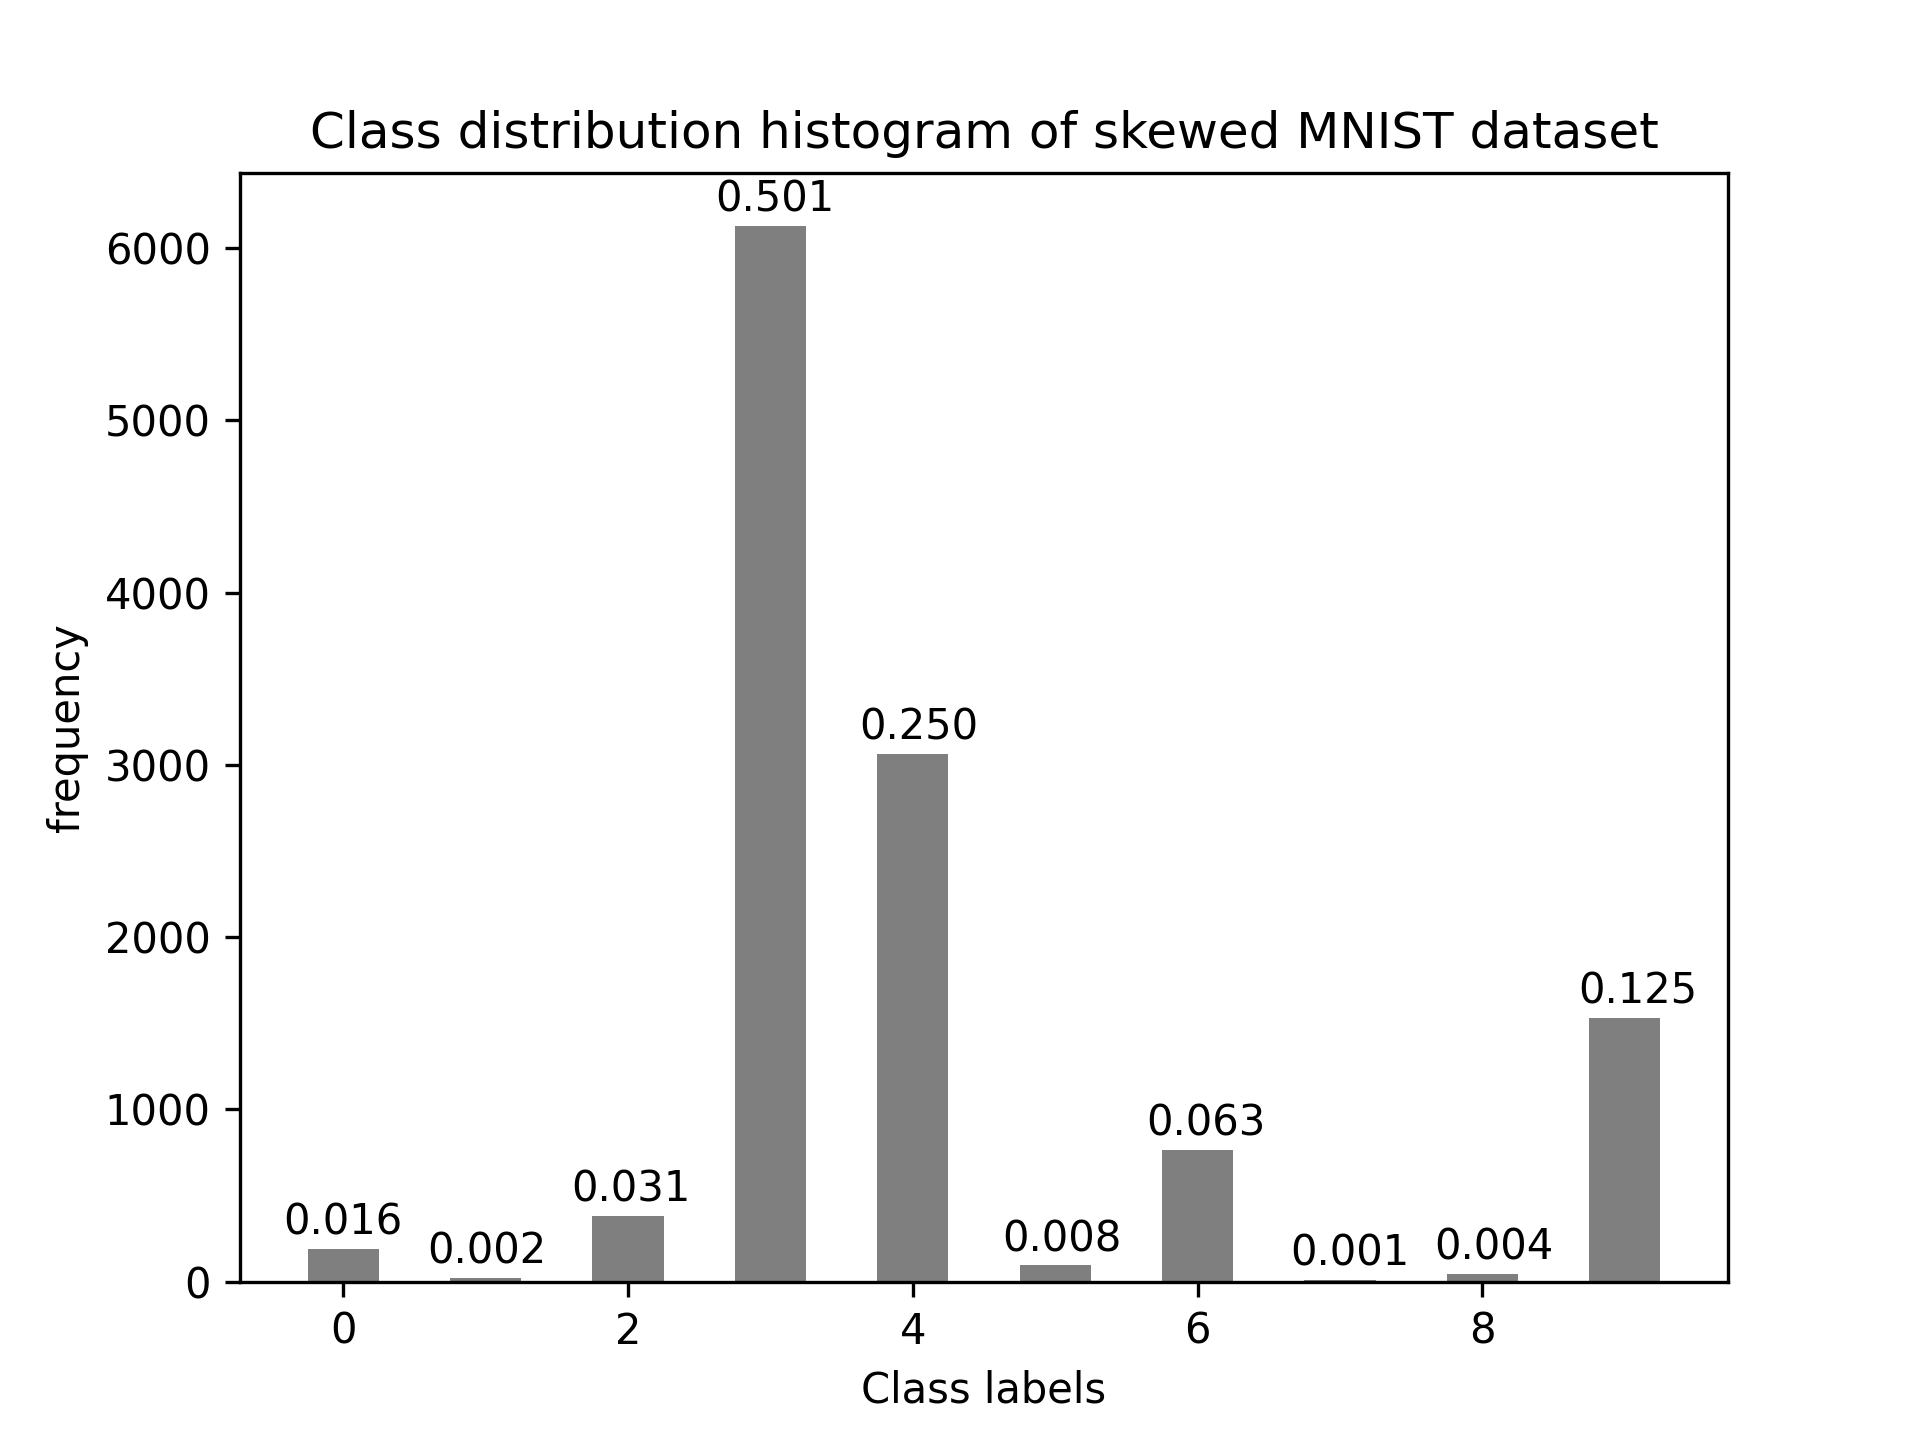
\includegraphics[width=0.5\textwidth]{class_histogram.png}
%\captionof{Histogram of True Classes\label{fig:histogram}}
\end{center}    


\begin{center}    
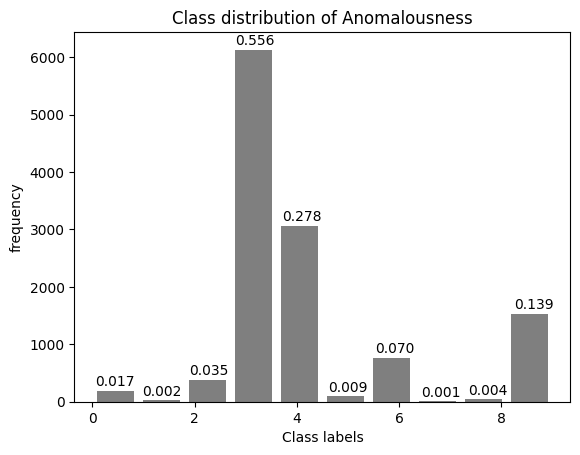
\includegraphics[width=0.5\textwidth]{class_histogram_anomalousness.png}
%\captionof{Histogram of Classification Results\label{fig:classification}}    
\end{center}
The accuracy of the method was 0.65485, or 65.5~\%.



    \let\clearpage\relax
    \section{Conclusion}
    
\section{Conclusion}

We were succesful in implementing an active learning algorithm to train a classifier on a dataset of 60000 samples using only a small set of those samples. 
The algorithm was able to reach a 95\% accuracy in far less than 1000 iterations.\par
The SVM classifier performed better than the Random Forest classifier in most cases. 
The highest uncertaintity query strategy was the most effective query strategy for the SVM classifier. 
The lowest vote strategy was the most effective query strategy for the Random Forest classifier. The random query strategy proved to be a quite effective query strategy for both classifiers. 
The entropy query strategy provided mixed results for each classifier.\par
Due to the size of the graphs, they are added to the appendix.

    \let\clearpage\relax
    \section{References}
    [1] van Engelen, J.E., Hoos, H.H. A survey on semi-supervised learning. Mach Learn 109, 373–440 (2020). https://doi.org/10.1007/s10994-019-05855-6\newline
[2] $https://scikit-learn.org/stable/auto\_examples/$\newline$classification/plot\_classifier\_comparison.html$\newline$\#sphx-glr-auto-examples-classification-plot-classifier-comparison-py$\newline
[3] Wang, W., Zhou, ZH. (2007). Analyzing Co-training Style Algorithms. In: Kok, J.N., Koronacki, J., Mantaras, R.L.d., Matwin, S., Mladenič, D., Skowron, A. (eds) Machine Learning: ECML 2007. ECML 2007. Lecture Notes in Computer Science(), vol 4701. Springer, Berlin, Heidelberg. $https://doi.org/10.1007/978-3-540-74958-5\_42$
 

\end{multicols}
\end{document}
